\chapter{N\"utzliche \LaTeX-Pakete}

\section{bchart.sty -- Erstellung einfacher Balkendiagramme}

Das Paket \texttt{bchart} wurde von Tobias Kuhn entwickelt\seFootcite{Vgl.}{}{Kuh:Bch} und bietet die M\"oglichkeit, auf einfache Art und Weise \textbf{horizontale Balkendiagramme}
zu erzeugen.\footnote{Der Hinweis auf dieses Paket stammt von Julia Lakatos -- vielen Dank.} Weitere Informationen 
zur Anwendung des Pakets lassen sich bei dem \gls{ctan} finden.\footnote{\url{http://www.ctan.org/tex-archive/macros/latex/contrib/bchart}}
\vref{quelltext-bsp-bchart} enth\"alt den Quelltext f\"ur das Balkendiagramm aus \vref{bsp-bchart}.

\begin{programm}[htbp]
\begin{lstlisting}[keywordstyle=\color{black},showstringspaces=false]
\begin{figure}[htbp]
\centering
\begin{bchart}[step=10,max=100,width=11cm,unit=\,\%]
\bcbar[label=Note {1,0} -- {1,5}]{7.69}
\smallskip
\bcbar[label={1,6} -- {2,5}]{42.31}
\smallskip
\bcbar[label={2,6} -- {3,5}]{23.08}
\smallskip
\bcbar[label={3,6} -- {4,0}]{15.38}
\smallskip
\bcbar[label={4,1} -- {5,0}]{11.53}
\end{bchart}
\caption{Verteilung der Klausurnoten 
\textsl{Einf\"uhrung in die Programmierung}
\label{bsp-bchart}}
\end{figure}
\end{lstlisting}
\caption{Quelltext zur Erzeugung des Balkendiagramms aus \vref{bsp-bchart}\label{quelltext-bsp-bchart}}
\end{programm}
\clearpage


\begin{figure}[htbp]
\centering
\begin{bchart}[step=10,max=100,width=11cm,unit=\,\%]
\bcbar[label=Note {1,0} -- {1,5}]{7.69}
\smallskip
\bcbar[label={1,6} -- {2,5}]{42.31}
\smallskip
\bcbar[label={2,6} -- {3,5}]{23.08}
\smallskip
\bcbar[label={3,6} -- {4,0}]{15.38}
\smallskip
\bcbar[label={4,1} -- {5,0}]{11.53}
\end{bchart}
\caption{Verteilung der Klausurnoten 
\textsl{Einf\"uhrung in die Programmierung}
\label{bsp-bchart}}
\end{figure}


\newcommand{\TikZ}{\textsf{Ti\textsl{k}Z}}
\section{tikz.sty -- Konstruktion nahezu beliebig komplexer Grafiken}

Das \TikZ{}-Paket wurde urspr\"unglich von Till Tantau\seFootcite{Vgl.}{}{Tan:tik} entwickelt und erlaubt 
die Konstruktion nahezu beliebig komplexer Grafiken. 
Die Entwicklung des Pakets erfolgt derzeit auf SourceForge unter \url{http://sourceforge.net/projects/pgf}.\seFootcite{Vgl.}{}{Tan:tik}%
\seFootcite{Vgl.}{}{FT:tik}
Eine Einf\"uhrung in die Erstellung von Grafiken mit \TikZ{} ist in dem Buch von Joachim Schlosser zu 
finden.\seFootcite{Vgl.}{Kapitel 8.2.2, S. 138 ff}{Sch:WAS} Eine ausf\"uhrliche mehr als 700 Seiten umfassende Dokumentation wurde von Till Tantau in 
Zusammenarbeit mit weiteren Autoren verfasst.\seFootcite{Vgl.}{}{Tan:man}

\clearpage
\vref*{quelltext-bsp-tikz} enth\"alt den Quelltext f\"ur die Grafik aus \vref{bsp-tikz}.

\begin{programm}[htbp]
\begin{lstlisting}[showstringspaces=false]
\begin{figure}[htbp]
\centering
%
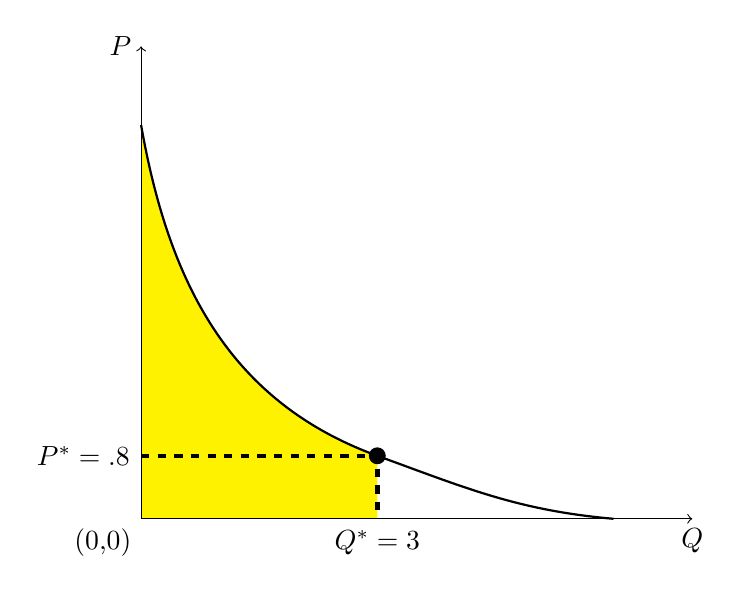
\begin{tikzpicture}
\path [fill=yellow] (0,0) -- (0,5) to [out=-80, in=160]
(3,.8) -- (3,0) -- (0,0);
\draw [<->] (0,6) node [left] {$P$} -- (0,0)
node [below left] {(0,0)} -- (7,0) node [below] {$Q$};
\draw [ultra thick, dashed] (0,.8) node [left] {$P^*=.8$} 
-- (3,.8) -- (3,0) node [below] {$Q^*=3$}; 
\draw [fill] (3,.8) circle (0.1);
\draw [thick] (0,5) to [out=-80, in=160] (3,.8) to
[out=-20, in=175] (6,0);
\end{tikzpicture}
%
\caption{Beispiel f\"ur eine mit \TikZ{} erstellte Grafik
\label{bsp-tikz}}
\end{figure}
\end{lstlisting}
\caption{Quelltext zur Erzeugung der Grafik aus \vref{bsp-tikz}\label{quelltext-bsp-tikz}}
\end{programm}



\begin{figure}[htbp]
\centering
%
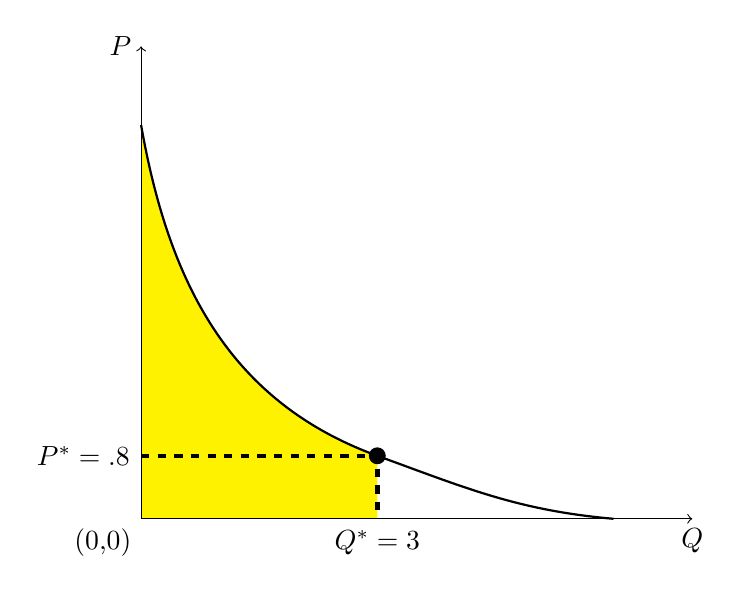
\begin{tikzpicture}
\path [fill=yellow] (0,0) -- (0,5) to [out=-80, in=160]
(3,.8) -- (3,0) -- (0,0);
\draw [<->] (0,6) node [left] {$P$} -- (0,0)
node [below left] {(0,0)} -- (7,0) node [below] {$Q$};
\draw [ultra thick, dashed] (0,.8) node [left] {$P^*=.8$} 
-- (3,.8) -- (3,0) node [below] {$Q^*=3$}; 
\draw [fill] (3,.8) circle (0.1);
\draw [thick] (0,5) to [out=-80, in=160] (3,.8) to
[out=-20, in=175] (6,0);
\end{tikzpicture}
%
\caption{Beispiel f\"ur eine mit \TikZ{} erstellte Grafik
\label{bsp-tikz}}
\end{figure}

\clearpage
\section{listings.sty -- Formatierung von Quelltexten}

Das Paket \texttt{listings.sty} wurde von Carsten Heinz und Brooks Moses entwickelt. Es unterst\"utzt f\"ur eine gro{\ss}e 
Menge von Programmiersprachen die Formatierung der Quelltexte.\seFootcite{Vgl.}{}{HM:lis} Die Liste der Sprachen reicht von 
ABAP bis XSLT.\seFootcite{Vgl.}{S. 12}{HM:lis}

Mit dem \texttt{lstset}-Kommando k\"onnen global f\"ur eine Programmiersprache die Formatierungsparameter definiert werden.
In \texttt{wa-konfiguration.tex} wurde beispielsweise festgelegt, dass standardm\"a{\ss}ig als Programmiersprache Java verwendet 
wird (\verb+language = Java+) und die Schl\"usselw\"orter blau darzustellen sind (\texttt{keywordstyle = \textbackslash{}color\{blue\}}).

F\"ur ein Listing lassen sich diese Eigenschaften \"uber optionale Parameter beim Start 
der \verb+lstlisting+-Umgebung umdefinieren. 


Bei \vref{bsp-zeilennummern} wurden statt \verb+\begin{lstlisting}+ einige optionale Parameter verwendet: \newline
\verb+\begin{lstlisting}[keywordstyle=\color{red},numbers=left,+\newline\verb+firstnumber=3,numbersep=5mm]+

\begin{seList}
\item \verb+firstnumber+ legt die erste Zeilennummer fest. Wird die Angabe von \verb+firstnumber+ weggelassen, 
dann wird der Standardwert 1 verwendet.
\item \verb+numbersep+ legt den Abstand zwischen der Zeilennummer und der ersten Spalte des Quelltextes fest. 
Fehlt die Angabe, dann wird der Standardwert 10pt benutzt.\seFootcite{Vgl.}{S. 31}{HM:lis}
\end{seList}

\begin{programm}[htbp]
\begin{lstlisting}[keywordstyle=\color{red},numbers=left,
firstnumber=3,numbersep=5mm]
public class HelloDHBW {
  public static void main ( String[] args ) {
    System.out.println ( "Hello DHBW" );
  } // main
} // HelloDHBW
\end{lstlisting}
\caption{Ausgabe eines Programms mit Zeilennummern und roten Schl\"usselw\"ortern\label{bsp-zeilennummern}}
\end{programm}

M\"ochte man verhindern, dass die Zeilennummern \"uber den linken Seitenrand hinausgehen, dann kann dieses mit 
dem optionalen Parameter \verb+xleftmargin+ erreicht werden. Beispielsweise liefert die zus\"atzliche Verwendung von 
\verb+xleftmargin=10mm+ die in \vref{bsp-leftmargin} dargestellte Formatierung.

\begin{programm}[htbp]
\begin{lstlisting}[numbers=left,
firstnumber=1,numbersep=5mm,xleftmargin=10mm]
public class HelloDHBW {
  public static void main ( String[] args ) {
    System.out.println ( "Hello DHBW" );
  } // main
} // HelloDHBW
\end{lstlisting}
\caption{Ausgabe eines Programms mit Zeilennummern sowie der 
Verwendung des optionalen Parameters \texttt{xleftmargin}\label{bsp-leftmargin}}
\end{programm}

Um f\"ur eine korrekte linksb\"undige Ausgabe der Zeilennummern nicht \textsl{\textbf{basteln}} zu m\"ussen, wird das neue 
Kommando \verb+\seListingLineNoConfig+ zur Verf\"ugung gestellt. Es besitzt vier Parameter:

\begin{seList}
\item Der erste Parameter ist (typischerweise) die \textbf{gr\"o{\ss}te Zeilennummer}, die in einem Listing auftritt. Hier\"uber wird die 
Breite ermittelt, die f\"ur die Zeilennummern ben\"otigt wird.\footnote{Prinzipiell reicht es aus, eine Zahl von 0 bis 9 anzugeben, wenn 
die gr\"o{\ss}te Zeilennummer einstellig ist, eine Zahl zwischen 10 und 99, wenn die gr\"o{\ss}te Zeilennummer zweistellig ist, usw.} Wenn f\"ur die 
Zeilennummern eine andere Schriftgr\"o{\ss}e oder eine spezielle Schriftart verwendet wird, dann sind die entsprechenden 
Schriftattribute ebenfalls mit anzugeben.
\item \"Uber den zweiten und dritten Parameter ist es m\"oglich, einen \textbf{Pr\"afix}- und \textbf{Postfixtext} f\"ur die Zeilennummern zu definieren. 
Beispielsweise k\"onnten die Zeilennummern in runde Klammern eingeschlossen werden. 
Wenn f\"ur die 
Zeilennummern eine andere Schriftgr\"o{\ss}e oder eine spezielle Schriftart verwendet wird, dann sind die entsprechenden 
Schriftattribute hier ebenfalls mit anzugeben.
\item Der vierte Parameter stellt den \textbf{Abstand zwischen der Zeilennummer und der ersten Spalte des Quelltextes} dar. Dieser Wert muss, 
um eine linksb\"undige Ausgabe der Zeilennummern zu erreichen, mit dem Wert \verb+numbersep+ \"ubereinstimmen.
\end{seList}

Mit dem Aufruf von \verb+\seListingLineNoConfig{13}{(}{)}{5mm}+ vor der Ausgabe des Quelltextes erreicht man die in \vref{bsp-linksbuendig} 
dargestellte Ausgabe der Zeilennummern, sofern bei \verb+\begin{lstlisting}+ gilt:

\begin{seList}
\item Der optionale Parameter \verb+firstnumber+ hat den Wert \verb+9+.
\item Der optionale Parameter \verb+numbersep+ hat den Wert \verb+5mm+.
\item Der optionale Paremeter \verb+xleftmargin+ hat den Wert \verb+\seListingLineNo+.\footnote{\texttt{\textbackslash{}seListingLineNo} wurde als 
\textsl{L\"angenregister} definiert. Das Kommando \texttt{\textbackslash{}se\-Lis\-ting\-Line\-No\-Con\-fig} berechnet den ben\"otigten Wert f\"ur \texttt{xleftmargin} und schreibt diesen 
Wert in das L\"angenregister.}
\end{seList}

\clearpage

\seListingLineNoConfig{13}{(}{)}{5mm}

\begin{programm}[htbp]
\begin{lstlisting}[numbers=left,firstnumber=9,numbersep=5mm,xleftmargin=\seListingLineNo]
public class HelloDHBW {
  public static void main ( String[] args ) {
    System.out.println ( "Hello DHBW" );
  } // main
} // HelloDHBW
\end{lstlisting}
\caption{Ausgabe eines Programms mit linksb\"undigen Zeilennummern\label{bsp-linksbuendig}}
\end{programm}


\section{supertabular.sty -- Mehrseitige Tabellen}

Das Paket \texttt{supertabular.sty} wurde von Johannes Braams und Theo Jurriens entwickelt.\seFootcite{Vgl.}{}{BJ:sup}
Neben der Erstellung mehrseitiger Tabellen bietet es im Vergleich zur \texttt{tabular}-Umgebung weitere Formatierungsm\"oglichkeiten.

Die wichtigsten Kommandos f\"ur mehrseitige Tabellen sind:\seFootcite{Vgl.}{S. 265}{MG:lat}

\begin{seList}
\item \texttt{\textbackslash{}tablehead\{{\textsl{zeilen}\}}} \newline
Der Parameter \textsl{zeilen} definiert die Tabellenzeilen, die am Kopf jeder Tabellenseite wiederholt werden.
\item \texttt{\textbackslash{}tablefirsthead\{{\textsl{zeilen}\}}} \newline
Wird neben \verb+tablehead+ auch \verb+tablefirsthead+ verwendet, so besteht die erste Tabellen\"uberschrift aus den 
Zeilen, die als Parameter \"uber \verb+\tablefirsthead+ festgelegt wurden. Auf allen Folgeseiten werden dann diejenigen 
Zeilen verwendet, die \"uber \verb+\tablehead+ definiert wurden.
\item \texttt{\textbackslash{}tabletail\{{\textsl{zeilen}\}}} \newline
Hiermit wird festgelegt, welche Zeilen am Ende einer Tabellenseite ausgegeben werden.
\item \texttt{\textbackslash{}tablelasttail\{{\textsl{zeilen}\}}} \newline
Mit \verb+\tablelasttail+ kann f\"ur die letzte Tabellenseite gesondert festgelegt werden, 
welche Zeilen auszugeben sind. 
\end{seList}

Die Angabe der Kommandos erfolgt vor der eigentlichen Verwendung der \texttt{su\-per\-ta\-bu\-lar}-Umgebung und wirkt sich auf alle 
folgenden Tabellen aus, die \"uber eine \texttt{su\-per\-ta\-bu\-lar}-Umgebung definiert werden. 

Da sich Gleitobjekte nicht \"uber mehrere Seiten erstrecken k\"onnen, ist es nicht sinnvoll, die \verb+supertabular+-Umgebung
mit der \verb+table+-Umgebung zu kombinieren. Um trotzdem eine Tabellenunterschrift erzeugen zu k\"onnen, stellt das 
\texttt{supertabular}-Paket eigene \verb+\caption+-Kommandos zur Verf\"ugung. Mit dem Kommando \texttt{\textbackslash{}bot\-tom\-cap\-tion} 
kann eine Tabellenunterschrift erzeugt werden, die auch in das Tabellenverzeichnis aufgenommen wird. Das \verb+\bottomcaption+-Kommando
muss ebenfalls vor dem Beginn der \verb+supertabular+-Umgebung angegeben werden.

In \vref{quelltext-bsp-supertabular} sind die Kommandos dargestellt, die f\"ur die Erzeugung der  \vref{bsp-supertabular} 
verwendet wurden. 

\begin{programm}[htbp]
\begin{lstlisting}[showstringspaces=false]
\tablefirsthead{\hline
   \multicolumn{2}{|c|}{\textbf{Gesamtumsatz 2012}}
   \\\hline\hline \textbf{Abteilung} 
   & \textbf{Umsatz}\\\hline}
\tablehead{\hline 
   \textbf{Abteilung} & \textbf{Umsatz}\\\hline}
\tabletail{\hline\multicolumn{2}{|r|}
   {\textsl{Fortsetzung n\"achste Seite}}\\\hline}
\tablelasttail{\hline
   \hline Gesamtumsatz & 148500,88\\\hline}
\bottomcaption{Jahresumsatz 2012\label{bsp-supertabular}}

\begin{center}%
\begin{supertabular}{ | l | r |}
Verkauf Industriemaschinen & 2100,55 \\
...
Verkauf 58 & 2100,55 \\
\end{supertabular}
\end{center}

\end{lstlisting}
\caption{Quelltext zur Erzeugung der \vref{bsp-supertabular}\label{quelltext-bsp-supertabular}}
\end{programm}

\tablefirsthead{\hline
   \multicolumn{2}{|c|}{\textbf{Gesamtumsatz 2012}}
   \\\hline\hline \textbf{Abteilung} 
   & \textbf{Umsatz}\\\hline}
\tablehead{\hline 
   \textbf{Abteilung} & \textbf{Umsatz}\\\hline}
\tabletail{\hline\multicolumn{2}{|r|}
   {\textsl{Fortsetzung n\"achste Seite}}\\\hline}
\tablelasttail{\hline
   \hline Gesamtumsatz & 148500,88\\\hline}
\bottomcaption{Jahresumsatz 2012\label{bsp-supertabular}}


%\tablefirsthead{\hline\multicolumn{2}{|c|}{\textbf{Gesamtumsatz 2012}}\\\hline\hline \textbf{Abteilung} & \textbf{Umsatz}\\\hline}
%\tablehead{\hline \textbf{Abteilung} & \textbf{Umsatz}\\\hline}
%\tabletail{\hline\multicolumn{2}{|r|}{\textsl{Fortsetzung n\"achste Seite}}\\\hline}
%\tablelasttail{\hline\hline Gesamtumsatz & 148500,88\\\hline}
%\bottomcaption{Jahresumsatz 2012\label{bsp-supertabular}}

\begin{center}%
\begin{supertabular}{ | l | r |}
Verkauf Industriemaschinen & 2100,55 \\
Verkauf 1 & 3020,17 \\
Verkauf 2 & 2100,55 \\
Verkauf 3 & 3020,17 \\
Verkauf 4 & 2100,55 \\
Verkauf 5 & 3020,17 \\
Verkauf 6 & 2100,55 \\
Verkauf 7 & 3020,17 \\
Verkauf 8 & 3020,17 \\
Verkauf 9 & 2100,55 \\
Verkauf 10 & 3020,17 \\
Verkauf 11 & 2100,55 \\
Verkauf 12 & 3020,17 \\
Verkauf 13 & 2100,55 \\
Verkauf 14 & 3020,17 \\
Verkauf 15 & 2100,55 \\
Verkauf 16 & 3020,17 \\
Verkauf 17 & 2100,55 \\
Verkauf 18 & 3020,17 \\
Verkauf 19 & 3020,17 \\
Verkauf 20 & 2100,55 \\
Verkauf 21 & 3020,17 \\
Verkauf 22 & 2100,55 \\
Verkauf 23 & 3020,17 \\
Verkauf 24 & 2100,55 \\
Verkauf 25 & 3020,17 \\
Verkauf 26 & 2100,55 \\
Verkauf 27 & 3020,17 \\
Verkauf 28 & 2100,55 \\
Verkauf 29 & 3020,17 \\
Verkauf 30 & 2100,55 \\
Verkauf 31 & 3020,17 \\
Verkauf 32 & 2100,55 \\
Verkauf 33 & 3020,17 \\
Verkauf 34 & 2100,55 \\
Verkauf 35 & 3020,17 \\
Verkauf 36 & 2100,55 \\
Verkauf 37 & 3020,17 \\
Verkauf 38 & 3020,17 \\
Verkauf 39 & 2100,55 \\
Verkauf 40 & 3020,17 \\
Verkauf 41 & 2100,55 \\
Verkauf 42 & 3020,17 \\
Verkauf 43 & 2100,55 \\
Verkauf 44 & 3020,17 \\
Verkauf 45 & 2100,55 \\
Verkauf 46 & 3020,17 \\
Verkauf 47 & 2100,55 \\
Verkauf 48 & 3020,17 \\
Verkauf 49 & 3020,17 \\
Verkauf 50 & 2100,55 \\
Verkauf 51 & 3020,17 \\
Verkauf 52 & 2100,55 \\
Verkauf 53 & 3020,17 \\
Verkauf 54 & 2100,55 \\
Verkauf 55 & 3020,17 \\
Verkauf 56 & 2100,55 \\
Verkauf 57 & 3020,17 \\
Verkauf 58 & 2100,55 \\
\end{supertabular}
\end{center}





